\documentclass[a4paper,12pt]{report}

% Packages nécessaires
\usepackage[utf8]{inputenc}  % Encodage des caractères
\usepackage[T1]{fontenc}     % Gestion des caractères spéciaux
\usepackage[francais]{babel} % Langue française
\usepackage{graphicx}        % Inclusion des images
\usepackage{hyperref}        % Liens hypertexte
\usepackage{geometry}        % Marges
\usepackage{xcolor}
\usepackage{float}
\usepackage{array}
\geometry{margin=1in}        % Définit des marges de 1 pouce

% images folder
\graphicspath{ {../images/} }

% Informations pour la page de titre
\title{
  
\includegraphics[width=10cm]{../images/logo-univ-evry} \\[1cm] % Logo avec chemin vers le fichier
  \textbf{Rapport projet scoring}
}
\author{DIEDHIOU Mamadou, HAOUD Anas, NGETH Laurent, PAZITHNOV Artemii}
\date{\today}

\begin{document}

% Page de titre
\maketitle

% Table des matières
\tableofcontents
\newpage

% Introduction
\chapter{Introduction}

Dans le monde financier, les institutions de prêt sont confrontées à un défi majeur : concilier la nécessité d'octroyer des crédits tout en minimisant le risque de défauts. 
Les prêts sur valeur domiciliaire, où l'emprunteur utilise la valeur nette de son bien immobilier comme garantie, jouent un rôle particulièrement important dans cet équilibre. 
Ces prêts offrent une flexibilité aux emprunteurs, que ce soit pour consolider des dettes ou financer des améliorations de leur habitation, mais ils exposent également les prêteurs à des pertes 
financières potentielles en cas de non-remboursement. Prédire quels emprunteurs sont susceptibles de faire défaut constitue donc une tâche essentielle pour les banques et institutions financières.

\bigbreak

Le jeu de données utilisé dans cette étude, HMEQ, fournit des informations sur 5 960 prêts sur valeur domiciliaire, incluant les caractéristiques des emprunteurs et les détails relatifs aux défauts de paiement.
Il capture divers facteurs influençant la solvabilité, tels que le montant du prêt demandé, le solde hypothécaire, la valeur de la propriété, la situation professionnelle, l’historique de crédit et le ratio dette-revenu.\\
La variable principale d’intérêt, BAD, indique si un emprunteur a fait défaut (1) ou a remboursé son prêt avec succès (0). 
Comprendre les relations entre ces variables et les résultats des prêts est essentiel pour améliorer l’évaluation du risque de crédit.

\bigbreak

Ce projet vise à développer un modèle prédictif pour BAD en utilisant des techniques d’apprentissage automatique, complétées par des analyses statistiques rigoureuses. 
En identifiant les principaux modèles et prédicteurs, ce modèle permettra aux prêteurs de prendre des décisions plus éclairées, réduisant les risques financiers tout en assurant un accès équitable au crédit. 
Le processus inclura une analyse exploratoire des données, un prétraitement, une sélection des modèles et une évaluation des performances. 
Une attention particulière sera accordée aux défis tels que le déséquilibre des classes, les valeurs aberrantes et les données manquantes, qui sont inhérents aux jeux de données réels.


% Chapitre 1
\chapter{Les données}
\section{Description des données}

\subsubsection{Variable dépendante (Target)}

La variable \textbf{BAD} représente la variable dépendante ou cible de l'analyse.
Elle est binaire et prend deux valeurs possibles :

\begin{itemize}
  \item 0 : indique que le client ne fait pas défaut.
  \item 1 : indique que le client fait défaut.
\end{itemize}

\bigbreak

\begin{figure}[h!]
  \begin{center}
    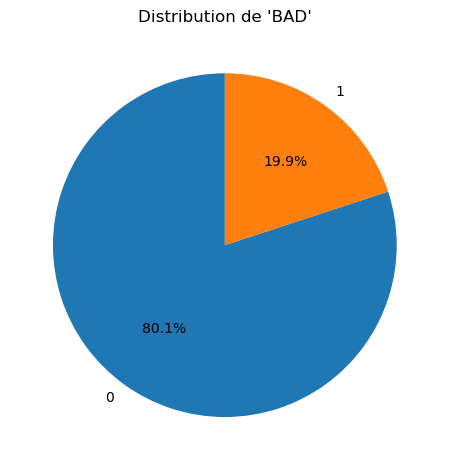
\includegraphics[width=0.5\textwidth]{../images/target_distribution}
  \end{center}
  \caption{Distribution de la variable Target "BAD"}
  \label{fig:dis_target}
\end{figure}


Le graphique en secteurs présenté (Figure \ref{fig:dis_target}) illustre la répartition des cas dans le dataset :
\begin{itemize}
  \item 80,1\% des clients appartiennent à la catégorie BAD = 0, ce qui signifie qu'ils n'ont pas fait défaut.
  \item 19,9\% des clients appartiennent à la catégorie BAD = 1, ce qui signifie qu'ils ont fait défaut.
\end{itemize}
\ \\

Cette distribution montre un déséquilibre notable entre les deux classes, avec une majorité de clients qui ne font pas défaut. 
Cela reflète une situation réaliste où les cas de défaut sont généralement moins fréquents dans une population de clients. \newline

La variable \textbf{BAD} est directement liée à l'objectif du projet, qui consiste probablement à prédire la probabilité qu'un client fasse défaut.
Cette information est cruciale pour la prise de décision dans des contextes tels que l'octroi de crédits ou la gestion du risque.

La nature binaire de la variable en fait une cible idéale pour des modèles de machine learning supervisés, tels que la régression logistique, 
les forêts aléatoires ou les réseaux de neurones, qui peuvent classifier les observations comme défaut (1) ou non défaut (0).

Une prédiction correcte de la variable BAD permet de mieux gérer les risques financiers en identifiant les clients susceptibles 
de faire défaut et en adaptant les stratégies en conséquence (par exemple, en ajustant les taux d'intérêt ou en refusant certains prêts).
\bigbreak
Bien que la variable soit déséquilibrée, cet aspect est intéressant car il reflète une réalité du domaine financier. Des techniques comme le suréchantillonnage, le sous-échantillonnage ou 
l'utilisation de métriques adaptées (comme le F1-score ou l'AUC-ROC) peuvent être utilisées pour traiter ce déséquilibre dans les analyses.

\subsubsection{Variables explicatives}

\begin{figure}[h!]
  \begin{center}
    \begin{tabular}{||c c p{10cm}||} 
     \hline
     Variable & Type & Description \\ [0.5ex] 
     \hline\hline
     LOAN & Numérique & Montant demandé dans le cadre du prêt \\ 
     \hline
     MORTDUE & Numérique & Montant restant dû sur l’hypothèque existante \\
     \hline
     VALUE & Numérique & Valeur estimée de la propriété utilisée comme garantie \\
     \hline
     REASON & Qualitative & Motif du prêt : DebtCon (consolidation de dettes) ou HomeImp (amélioration de l’habitat) \\
     \hline
     JOB & Qualitative & Catégorie professionnelle de l’emprunteur \\
     \hline
     YOJ & Numérique & Ancienneté dans l’emploi actuel, exprimée en années \\
     \hline
     DEROG & Numérique & Nombre de rapports dérogatoires majeurs associés à l’emprunteur \\
     \hline
     DELINQ & Numérique & Nombre de lignes de crédit en retard de paiement \\
     \hline
     CLAGE & Numérique & Âge de la plus ancienne ligne de crédit, exprimé en mois \\
     \hline
     NINQ & Numérique & Nombre de demandes de crédit récentes effectuées par l’emprunteur \\
     \hline
     CLNO & Numérique & Nombre total de lignes de crédit détenues par l’emprunteur \\
     \hline
     DEBTINC & Numérique & Ratio dette-revenu : indicateur du poids de la dette par rapport aux revenus de l’emprunteur \\ [1ex] 
     \hline
    \end{tabular}
  \end{center}
  \caption{Tableau des descriptions des variables}
  \label{fig:tab_vif_num_num}
\end{figure}

\begin{enumerate}
  \item{ \textbf{Variables Numériques :}\newline
    Les variables telles que {\color{teal} LOAN}, {\color{teal} MORTDUE}, et {\color{teal} VALUE} fournissent une mesure directe de la situation financière des emprunteurs, notamment leur exposition à la dette et la valeur de leurs actifs. 
    Les variables {\color{teal} DEROG}, {\color{teal} DELINQ}, et {\color{teal} NINQ} permettent d’évaluer l’historique de crédit et le comportement récent des emprunteurs vis-à-vis des obligations financières.
    Enfin, le ratio {\color{teal} DEBTINC} constitue un indicateur essentiel de la capacité de remboursement d’un individu.
  }
  \item{ \textbf{Variables Qualitatives :}\newline
    Les variables catégorielles {\color{teal} REASON} et {\color{teal} JOB} apportent un contexte supplémentaire en décrivant les motivations des emprunteurs et leur situation professionnelle, deux facteurs pouvant influencer le risque de défaut de paiement. 
    La variable cible BAD, en tant que variable binaire, servira à évaluer la performance des modèles prédictifs.
  }
  \item{ \textbf{Limites et Enjeux :}\newline
    Bien que les données soient riches en variables financières, elles manquent de certaines informations socio-démographiques, telles que l’état matrimonial ou la situation géographique, qui pourraient améliorer la précision des prédictions. 
    De plus, la gestion des valeurs manquantes, notamment pour des variables comme {\color{teal} DEBTINC}, sera un aspect déterminant dans le prétraitement des données.
  }
\end{enumerate}

\section{Visualisation}

\subsubsection{Variables numériques}

Le graphique en Annexe \ref{fig:plot_dist_num_data} représente la distribution des variables numériques.

Cependant, la présence de valeurs extrêmes montre une sous-population gérant des montants significativement plus élevés, probablement associée à des revenus plus importants ou à des cas atypiques.
Cette disparité met en évidence une population diversifiée, allant de ceux avec une activité financière limitée à ceux ayant des engagements financiers ou des actifs considérables.

\bigbreak

Les variables liées au crédit, comme DEROG, DELINQ et NINQ, décrivent une population globalement responsable sur le plan financier.\\
La majorité des individus n’ont aucun rapport de crédit dérogatoire, peu de lignes de crédit en retard, et un faible nombre de demandes récentes de crédit.\\
Ces schémas reflètent un groupe ayant un comportement financier stable.
Toutefois, la présence de valeurs extrêmes, par exemple, plusieurs retards ou rapports dérogatoires révèle une petite sous-population à risque plus élevé, potentiellement en difficulté financière.\\
De manière similaire, le ratio dette/revenu (DEBTINC) soutient cette tendance, avec la majorité des individus maintenant des niveaux de dette gérables par rapport à leurs revenus, bien qu’une minorité affiche des ratios significativement plus élevés, suggérant une possible tension financière.

\bigbreak

Les variables liées à la maturité financière, telles que YOJ (années dans l’emploi actuel) et CLAGE (ancienneté de la ligne de crédit la plus vieille), révèlent que la majorité des individus ont des carrières professionnelles plus courtes et des historiques de crédit récents. \\
Cela pourrait indiquer une population plus jeune ou des individus ayant une expérience financière limitée.\\
Cependant, la présence de dossiers de crédit plus anciens et de carrières professionnelles plus longues pour certains reflète un mélange d’individus jeunes et plus établis financièrement.

\bigbreak

La variable CLNO, représentant le nombre de lignes de crédit, se distingue par une répartition plus équilibrée, avec une distribution proche de la normale.\\
Cela montre que la majorité des individus maintiennent un nombre modéré de lignes de crédit, reflétant une utilisation stable et responsable du crédit.

\bigbreak

Ce jeu de données reflète principalement une population stable financièrement, avec une petite sous-population à risque plus élevé en raison de valeurs extrêmes dans les niveaux d’endettement, l’historique de crédit ou les montants des prêts.\\
Cette répartition met en lumière des opportunités de segmentation et d’analyses plus approfondies pour mieux comprendre les comportements et caractéristiques des groupes majoritaires et des sous-groupes à risque.


\subsubsection{Boxplot et Outliers}

Les boxplots en Annexe \ref{fig:boxplot_var_num} illustrent des tendances significatives entre les variables financières et la variable cible BAD (0 ou 1). Ici, les clients qui font défaut (BAD = 1) sont comparés à ceux qui n’ont pas de problème de remboursement (BAD = 0).\\
Pour de nombreuses variables, on observe des différences marquées entre ces deux groupes.
Par exemple, les variables comme LOAN (montant du prêt) et MORTDUE (hypothèques dues) présentent des médianes plus élevées pour les clients qui font défaut, ce qui suggère que des niveaux d'endettement plus importants sont souvent associés à un risque accru de défaut.\\
De plus, des variables comme DEROG (litiges financiers) et DELINQ (retards de paiement) montrent des valeurs plus fréquentes et élevées pour les clients qui font défaut, ce qui en fait des indicateurs fiables de risque.

\bigbreak

Par ailleurs, les variables liées à la stabilité financière, comme YOJ (durée d’emploi) et CLAGE (ancienneté du crédit), révèlent que les clients qui font défaut ont généralement une ancienneté professionnelle ou financière plus courte.\\
Enfin, des indicateurs tels que DEBTINC (ratio dette/revenu) et NINQ (nombre de demandes récentes de crédit) affichent des niveaux significativement plus élevés pour les clients qui font défaut, renforçant leur pertinence comme signaux de risque financier.\\
Cette analyse met en lumière les variables les plus utiles pour prédire le défaut de paiement, aidant ainsi à affiner les modèles d’évaluation de crédit et à mieux comprendre les profils de risque des emprunteurs.

\pagebreak

\subsubsection{Variables catégorielles}

Nous pouvons clairement voir dans les barplots en Annexe \ref{fig:barplot_job_by_bad} et Annexe \ref{fig:barplot_reason_by_bad} que les variables catégorielles
possèdent plusieurs groupes. Ceux-ci peuvent être comptés et regroupés dans les différentes classes de la variable dépendante BAD, c'est-à-dire le groupe 0 ou 1.\\
On voit que certaines catégories sont plus représentées que d'autres. Nous devons en tenir compte lors du traitement des valeurs manquantes.\\
Ainsi, lorsque nous traitons des valeurs aberrantes, nous devons être prudents lorsque nous abandonnons l'observation avec la raison DEBTCON.


\section{NaN values}

\subsection{Variables numériques}

\begin{figure}[h!]
  \begin{center}
    \begin{tabular}{||c c c c c||} 
     \hline
     Feature & Null count & Overall \% & BAD=0 \% & BAD=1 \%\\ [0.5ex]
     \hline
     MORTDUE & 518 & 8.70\% & 8.63\% & 8.91\% \\
     \hline
     VALUE & 112 & 1.88\% & 0.14\% & 8.83\% \\
     \hline
     YOJ & 515 & 8.64\% & 9.43\% & 5.46\% \\
     \hline
     DEROG & 708 & 11.87\% & 13.01\% & 7.31\% \\
     \hline
     DELINQ & 580 & 9.73\% & 10.64\% & 6.05\% \\
     \hline
     CLAGE & 308 & 5.15\% & 4.82\% & 6.56\% \\
     \hline
     NINQ & 510 & 8.55\% & 9.11\% & 6.30\% \\
     \hline
     CLNO & 222 & 3.72\% & 3.54\% & 4.45\% \\
     \hline
     DEBTINC & 1257 & 21.26\% & 10.08\% & 66.10\% \\ [1ex] 
     \hline
    \end{tabular}
  \end{center}
  \caption{Tableau des VIF des variables numériques après suppression de "VALUE"}
  \label{fig:tab_nan_count_num_var}
\end{figure}

\bigbreak

D'après la Figure \ref{fig:tab_nan_count_num_var} calculé, toutes les variables numériques ont entre 1 et 20\% de valeurs manquantes.\\


\subsection{Variables catégorielles}

Au niveau des valeurs catégorielles, nous pouvons voir leur répartition dans un diagramme en camembert Figure \ref{fig:dist_missing_values_cat}.\\
Nous verrons dans la section suivante, comment nous les avons traités car, en effet, leur nombre est assez négligeable par rapport à la quantité totale d'observations.


% Chapitre 2
\chapter{Data processing}

\section{Traitement des valeurs nulles/extrèmes/manquantes}

\subsection{Variables numériques : Imputation par valeur calculée}

Lors de l’analyse exploratoire des données, nous avons identifié des valeurs manquantes au sein de plusieurs variables numériques.\\
Pour remédier à ce problème, nous avons appliqué trois méthodes d’imputation couramment utilisées, puis comparé leurs performances afin de sélectionner la méthode la plus adaptée.
Les méthodes d’imputation testées sont les suivantes :

\bigbreak

\begin{itemize}
  \item{ \textbf{Imputation par la moyenne :} \newline
    Cette méthode consiste à remplacer les valeurs manquantes par la moyenne des valeurs observées pour une variable donnée.\\
    Bien qu’elle soit simple à implémenter, elle peut être sensible aux valeurs extrêmes (outliers), ce qui peut biaiser les résultats.
  }
  \item{ \textbf{Imputation par la médiane :} \newline
    Cette méthode remplace les valeurs manquantes par la médiane des valeurs observées pour une variable donnée.\\
    Contrairement à la moyenne, la médiane est robuste face aux valeurs extrêmes et est souvent préférée dans les distributions asymétriques.
  }
  \item{ \textbf{Imputation par K-Nearest Neighbors (KNN) :} \newline
    Cette méthode utilise les valeurs des observations les plus proches (en termes de distance   calculée dans l’espace des variables) pour imputer les valeurs manquantes.\\
    Elle permet de capturer des relations locales et structurelles dans les données, ce qui peut produire des imputations plus précises.
  }
\end{itemize}

\bigbreak

Pour évaluer ces méthodes, nous avons appliqué chacune d'elles à nos données et comparé les distributions des variables après imputation avec leur distribution initiale (avant imputation).
Ces distributions ont été visualisées pour plusieurs variables afin d’observer l’impact de chaque méthode sur la structure des données, Figure \ref{fig:plot_num_imputation_distrib}.

\begin{figure}[h!]
  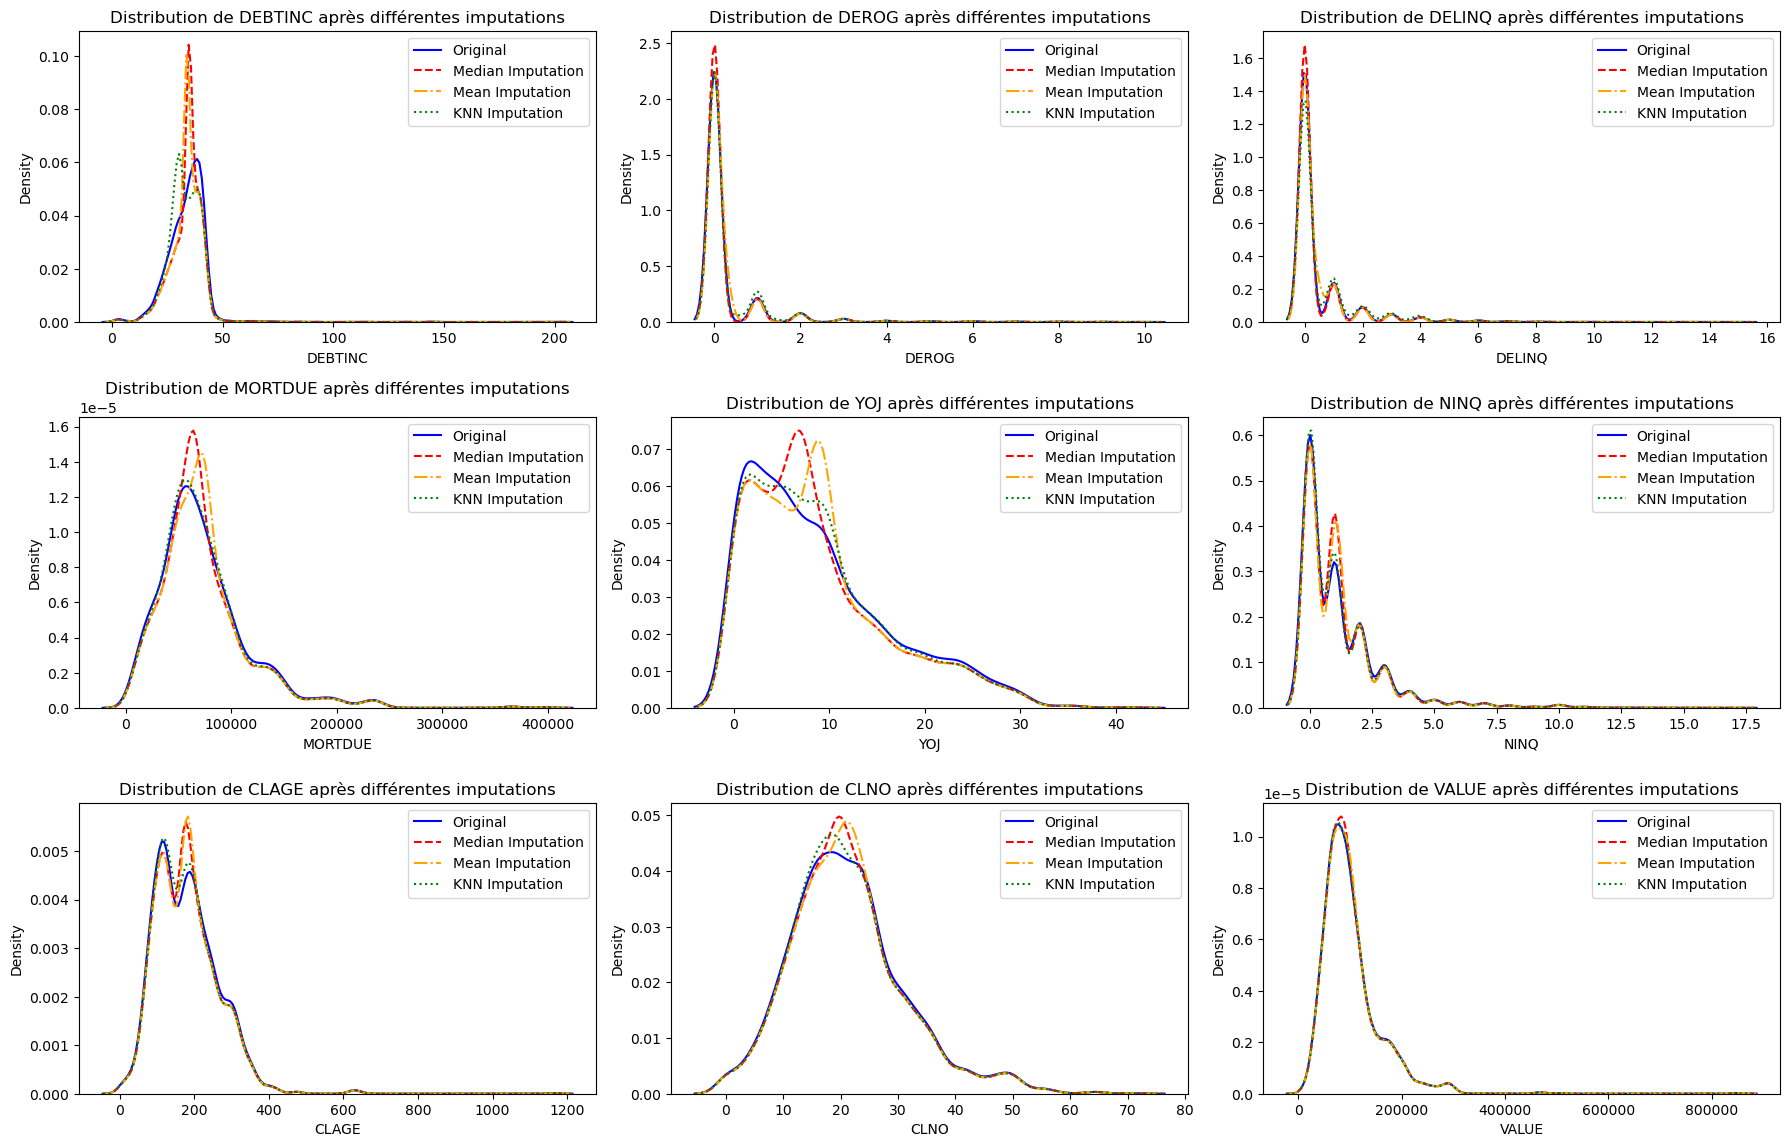
\includegraphics[width=\textwidth]{../images/plot_num_imputation_distrib}
  \caption{Distribution des variables numériques après différentes techniques d'imputations}
  \label{fig:plot_num_imputation_distrib}
\end{figure}

\pagebreak

Pour donner suite à cette comparaison, nous avons constaté que l’imputation par \textbf{KNN} était la méthode la plus adaptée dans notre cas.\\
Elle préserve au mieux la structure des distributions initiales des variables, contrairement aux méthodes par la moyenne ou la médiane, qui introduisent davantage de déviations, notamment pour les variables asymétriques ou contenant des valeurs extrêmes.
Ainsi, nous avons retenu l’imputation par \textbf{KNN} comme méthode définitive pour le traitement des valeurs manquantes dans les variables numériques. Ce choix garantit une meilleure qualité des données pour les étapes d’analyse et de modélisation à venir.

\subsection{Variables catégorielles : Imputation de données}

D'après la répartition des valeurs manquantes dans les variables catégorielles, on voit qu'elles 
uniquement présentes dans "REASON" et "JOB" (Figure \ref{fig:dist_missing_values_cat}).

\pagebreak

\begin{figure}[h!]
  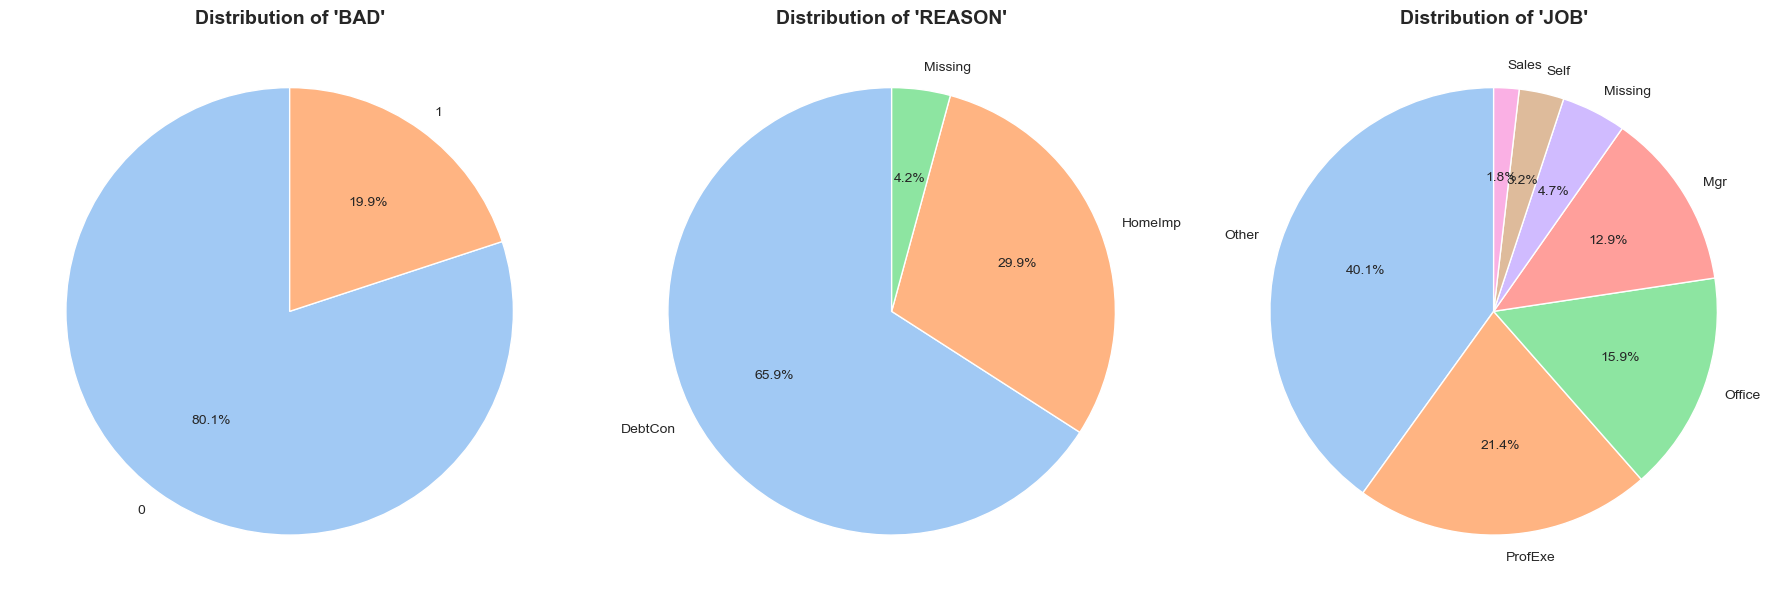
\includegraphics[width=\textwidth]{../images/piechart_valeurs_manquantes_var_categorial}
  \caption{Distribution des valeurs manquantes dans les variables catégorielles}
  \label{fig:dist_missing_values_cat}
\end{figure}

On voit que ces valeurs manquantes représentent aux alentours de 5\% des observations pour les variables "REASON" et "JOB".\\
\\
Nous avons choisi de réaliser une suppression des observations qui possèdent ces 2 variables catégorielles à nulles (Figure \ref{fig:dist_missing_values_cat_dropna}).\\
En effet, pour seulement 5\% des observations, il n'est pas nécessaire de vouloir combler les valeurs manquantes par une interpolation
sachant que cela peut induire davantage de biais dans nos données.\\
Nous avons déjà fait une imputation par KNN pour les valeurs numériques, de ce fait, nous jugeons que cela n'est pas nécessaire vu la quantité de données,
pour les variables catégorielles.

\begin{figure}[h!]
  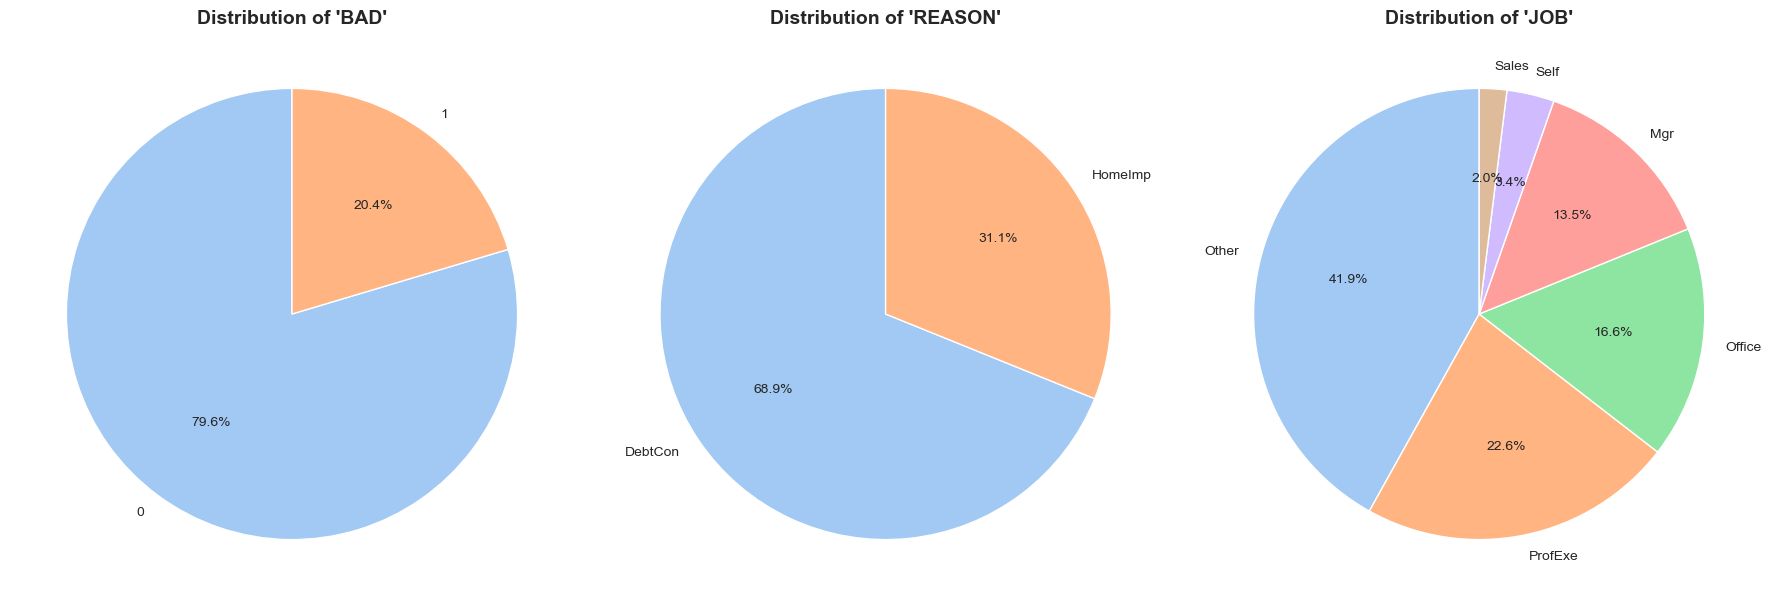
\includegraphics[width=\textwidth]{../images/piechart_valeurs_manquantes_var_categorial_dropna}
  \caption{Distribution des valeurs manquantes dans les variables catégorielles après suppression des observations avec NaN}
  \label{fig:dist_missing_values_cat_dropna}
\end{figure}


\chapter{Modélisation}

\section{Sélection des variables}

\subsection{Corrélation entre variable numérique-numérique}

À cette étape, il est important de bien sélectionner les variables explicatifs ayant un pouvoir relationnel avec la variable dépendante.\\
C'est pourquoi, nous analysons le tableau de corrélation entre les variables numériques de notre dataset (Figure \ref{fig:tab_corr_num_num}).

\begin{figure}[h!]
  \begin{center}
    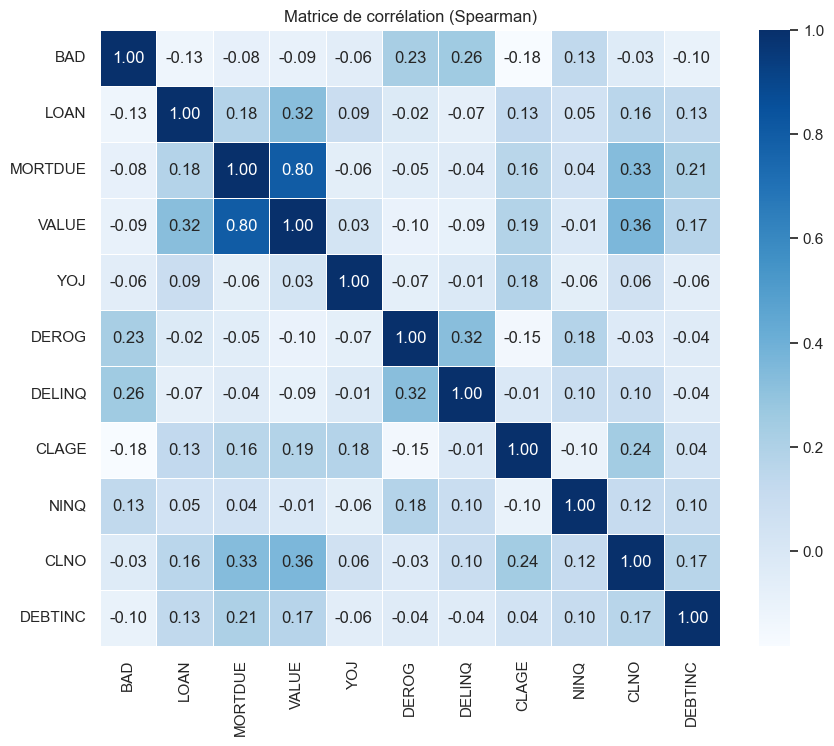
\includegraphics[width=0.8\textwidth]{../images/tab_corr_num_num}
  \end{center}
  \caption{Tableau de corrélation des variable numérique}
  \label{fig:tab_corr_num_num}
\end{figure}

Nous voyons que seules 2 variables explicatives, "VALUE" et "MORTDUE", ont une forte corrélation entre elles.\\
Une valeur aussi grande de 0.80 signifie qu'il y a une forte relation linéaire entre ces 2 variables. Nous sommes possiblement dans un cas de colinéarité.
On se demande donc s'il porte la même information vis-à-vis de la variable dépendante "BAD", auquel cas, il serait pertinent d'enlever une des 2 variables du modèle
afin d'éliminer la redondance d'informations.\\
\\
Mais pour confirmer nos soupçons, nous allons calculé le Variance Inflation Factor (VIF), un indicateur de multicolinéarité (Figure \ref{fig:tab_vif_num_num}).

\begin{figure}[h!]
  \begin{center}
    \begin{tabular}{||c c c||} 
     \hline
      & Feature & VIF \\ [0.5ex] 
     \hline\hline
     1 & LOAN & 4.378617 \\ 
     \hline
     2 & MORTDUE & 10.888010 \\
     \hline
     3 & VALUE & 11.658782 \\
     \hline
     4 & YOJ & 2.578970 \\
     \hline
     5 & DEROG & 1.194198 \\
     \hline
     6 & DELINQ & 1.296263 \\
     \hline
     7 & CLAGE & 5.665235 \\
     \hline
     8 & NINQ & 1.565770 \\
     \hline
     9 & CLNO & 6.614832 \\
     \hline
     10 & DEBTINC & 8.907927 \\ [1ex] 
     \hline
    \end{tabular}
  \end{center}
  \caption{Tableau des VIF des variables numériques}
  \label{fig:tab_vif_num_num}
\end{figure}

Les valeurs de VIF pour "MORTDUE" et "VALUE" nous confirment bien la présence d'une colinéarité avec les autres variables.\\
Le tableau précédent nous confirment que c'est bien ces deux variables les fautifs, nous décidons alors d'enlever au moins une de ces 2 variables
du modèle. Laquelle ?\\
\\
Nous voyons dans la Figure \ref{fig:tab_corr_num_num} que ces 2 variables ont approximativement (à 0.01 près) le même
niveau de corrélation avec la variable dépendante "BAD". De ce fait, il serait plus préférable de baser notre choix sur la valeur VIF la plus grande
car cela nous permettrait de supprimer le maximum de covariance entre les variables explicatives.\\
Sur ce critère, le choix de porte donc sur la variable \textbf{"VALUE"}.\\
\\

Ainsi, nous obtenons un nouveau tableau de corrélation (Figure \ref{fig:tab_corr_num_num_after_1st_drop}) et le nouveau
tableau des VIF (Figure \ref{fig:tab_vif_num_num_after_1st_drop}).\\

\begin{figure}[h!]
  \begin{center}
    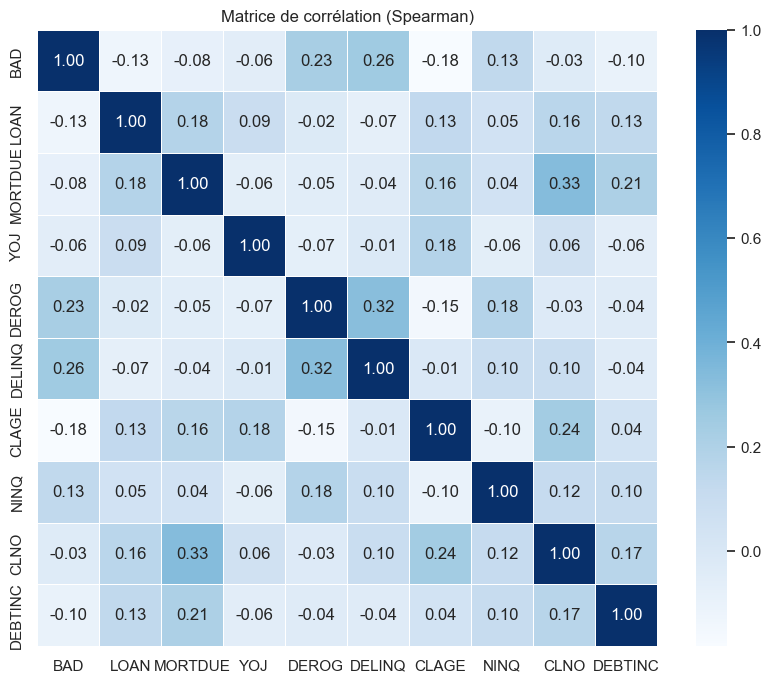
\includegraphics[width=0.8\textwidth]{../images/tab_corr_num_num_after_1st_drop}
  \end{center}
  \caption{Tableau de corrélation des variable numérique après suppression de "VALUE"}
  \label{fig:tab_corr_num_num_after_1st_drop}
\end{figure}

\begin{figure}[h!]
  \begin{center}
    \begin{tabular}{||c c c||} 
     \hline
      & Feature & VIF \\ [0.5ex] 
     \hline\hline
     1 & LOAN & 4.378617 \\ 
     \hline
     2 & MORTDUE & 10.888010 \\
     \hline
     3 & YOJ & 2.578970 \\
     \hline
     4 & DEROG & 1.194198 \\
     \hline
     5 & DELINQ & 1.296263 \\
     \hline
     6 & CLAGE & 5.665235 \\
     \hline
     7 & NINQ & 1.565770 \\
     \hline
     8 & CLNO & 6.614832 \\
     \hline
     9 & DEBTINC & 8.907927 \\ [1ex] 
     \hline
    \end{tabular}
  \end{center}
  \caption{Tableau des VIF des variables numériques après suppression de "VALUE"}
  \label{fig:tab_vif_num_num_after_1st_drop}
\end{figure}

\clearpage

Avec cette logique, nous continuons notre recherche de variables colinéaires en émettant des critères plus restrictifs :

\begin{itemize}
  \item Corrélation > 0.3 \textbf{ET}
  \item VIF > 5
\end{itemize}
\ \\

Avec ces critères, nous nous retrouvons avec de forte multicolinéarité entre LOAN, MORTDUE, CLNO et DEBTINC.\\
Au niveau de l'interprétation, on arrive à trouver facilement la variable "fautive" qui est DEBTINC (dont le VIF est le plus élevé, 8.99). C'est elle qui est fortement liées avec les autres variables et cela fait sens car :
\begin{itemize}
  \item LOAN : Les prêts plus importants augmentent généralement la dette totale, ce qui influence le ratio dette/revenu. 
  \item MORTDUE : L'encours des prêts hypothécaires contribue de manière significative à l'endettement total.  
  \item CLNO : Un nombre plus élevé de lignes de crédit peut indiquer un endettement plus important, ce qui a un impact sur le rapport dette/revenu.  
\end{itemize}

De ces faits, supprimer la variable "DEBTINC" de nos données pourraient diminuer les effets non désirés entre les variables explicatives.\\
Et c'est visiblement le cas avec ces nouveaux tableaux des indicateurs de corrélation (Figure \ref{fig:tab_corr_num_num_intermediary}) et de VIF (Figure \ref{fig:tab_vif_num_num_intermediary}).

\begin{figure}[h!]
  \begin{center}
    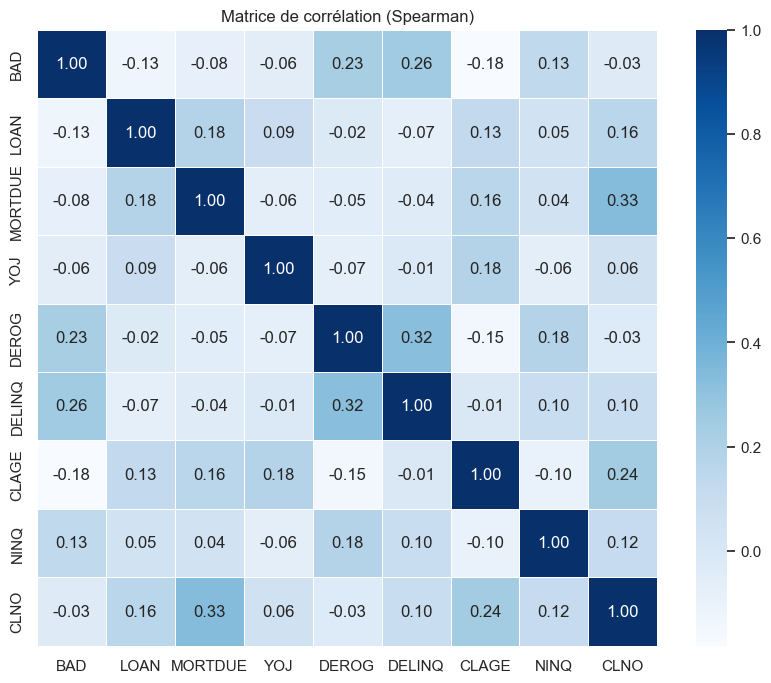
\includegraphics[width=0.8\textwidth]{../images/tab_corr_num_num_intermediary}
  \end{center}
  \caption{Tableau de corrélation des variable numérique après suppression de "DEBTINC"}
  \label{fig:tab_corr_num_num_intermediary}
\end{figure}

\begin{figure}[h!]
  \begin{center}
    \begin{tabular}{||c c c||} 
     \hline
      & Feature & VIF \\ [0.5ex] 
     \hline\hline
     1 & LOAN & 3.774757 \\ 
     \hline
     2 & MORTDUE & 4.361081 \\
     \hline
     3 & YOJ & 2.472750 \\
     \hline
     4 & DEROG & 1.188133 \\
     \hline
     5 & DELINQ & 1.293454 \\
     \hline
     6 & CLAGE & 5.205491 \\
     \hline
     7 & NINQ & 1.509163 \\
     \hline
     8 & CLNO & 5.909883 \\ [1ex] 
     \hline
    \end{tabular}
  \end{center}
  \caption{Tableau des VIF des variables numériques après suppression de "DEBTINC"}
  \label{fig:tab_vif_num_num_intermediary}
\end{figure}

Sur la même logique, l'indicateur VIF pour le CLAGE et le CLNO est supérieur à 5, ce qui peut s'expliquer logiquement compte tenu de la nature des deux variables.\\
Nous décidons de conserver CLAGE et d'abandonner CLNO car la première est plus corrélée à la caractéristique cible (-0.18 pour "CLAGE" contre -0.03 pour "CLNO").\\
\\
Ainsi nous obtenons le tableau de corrélation final (Figure \ref{fig:tab_corr_num_num_final}) et le tableau de VIF final (Figure \ref{fig:tab_vif_num_num_final}).

\begin{figure}[h!]
  \begin{center}
    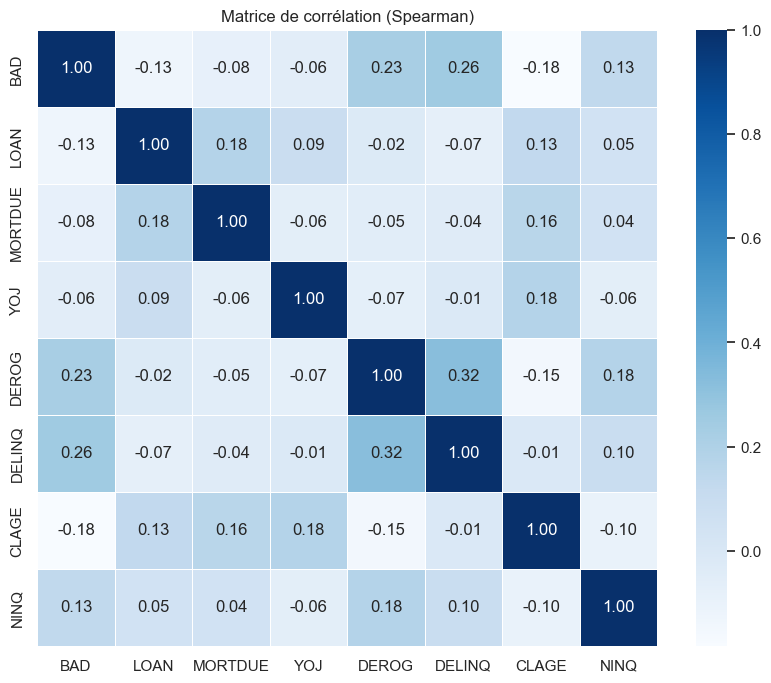
\includegraphics[width=0.8\textwidth]{../images/tab_corr_num_num_final.png}
  \end{center}
  \caption{Tableau de corrélation des variable numérique final}
  \label{fig:tab_corr_num_num_final}
\end{figure}

\begin{figure}[h!]
  \begin{center}
    \begin{tabular}{||c c c||} 
     \hline
      & Feature & VIF \\ [0.5ex] 
     \hline\hline
     1 & LOAN & 3.724226 \\ 
     \hline
     2 & MORTDUE & 3.643924 \\
     \hline
     3 & YOJ & 2.429276 \\
     \hline
     4 & DEROG & 1.182331 \\
     \hline
     5 & DELINQ & 1.253890 \\
     \hline
     6 & CLAGE & 4.412731 \\
     \hline
     7 & NINQ & 1.476348 \\ [1ex] 
     \hline
    \end{tabular}
  \end{center}
  \caption{Tableau des VIF des variables numériques final}
  \label{fig:tab_vif_num_num_final}
\end{figure}

Finalement, toutes nos variables respectent nos critères de non corrélation.
Nous gardons donc ces variables explicatives numériques dans notre modèle.


\subsection{Corrélation entre variable catégorielle-numérique}

Pour mesurer les corrélations entre les variables catégorielle et les variables numériques,
nous choisissons d'utilier l'ANalyse Of VAriance (ANOVA).\\

Lorsque nous analysons les variances des variables numériques par rapport à la variable dépendante "BAD", nous obtenons le tableau ANOVA ci-dessous (\ref{fig:anova_bad_cat_on_nums}).
\subsubsection{ANOVA: BAD <-- LOAN, MORTDUE, YOJ, DEROG, DELINQ, CLAGE, NINQ}

\begin{figure}[h!]
  \begin{center}
    \begin{tabular}{||c c c||} 
     \hline
     Category & Statistique F & p-value \\ [0.5ex] 
     \hline\hline
     LOAN & 43.611845 & 4.378365e-11 \\ 
     \hline
     MORTDUE & 17.150873 & 3.503906e-05 \\
     \hline
     YOJ & 18.897293 & 1.404214e-05 \\
     \hline
     DEROG & 353.561190 & 1.651631e-76 \\
     \hline
     DELINQ & 535.645619 & 3.412949e-113 \\
     \hline
     CLAGE & 160.690711 & 2.546471e-36 \\
     \hline
     NINQ & 143.898866 & 9.497433e-33 \\ [1ex] 
     \hline
    \end{tabular}
  \end{center}
  \caption{ANOVA des variables explicatives par rapport à "BAD"}
  \label{fig:anova_bad_cat_on_nums}
\end{figure}

Rappelons les hypothèses des tests d'indépendances entre 2 variables $x$ et $y$ :

\begin{itemize}
  \item H0 : $x$ est indépendante de $y$  
  \item H1 : $x$ est dépendante de $y$
\end{itemize}
\ \\
Lorsqu'on plot la significativité des variables explicatives numériques avec la variable dépendante "BAD", toutes les p-values sont nettement inférieures à 1\%.  
On peut donc rejeter à 1\% toutes les hypothèses H0 selon laquelle les variables explicatives sont indépendantes de la variable "BAD".\\
On laisse donc toutes ces variables explicatives numériques dans notre modèle.


\subsubsection{ANOVA: REASON <-- LOAN, MORTDUE, YOJ, DEROG, DELINQ, CLAGE, NINQ }

\begin{figure}[h!]
  \begin{center}
    \begin{tabular}{||c c c||} 
     \hline
     Category & Statistique F & p-value \\ [0.5ex] 
     \hline\hline
     LOAN & 220.022855 & 7.676688e-49 \\ 
     \hline
     MORTDUE & 3.973582 & 4.626836e-02 \\
     \hline
     YOJ & 8.628049 & 3.323912e-03 \\
     \hline
     DEROG & 0.242414 & 6.224878e-01 \\
     \hline
     DELINQ & 0.018321 & 8.923356e-01 \\
     \hline
     CLAGE & 17.075163 & 3.645952e-05 \\
     \hline
     NINQ & 85.510913 & 3.219899e-20 \\ [1ex] 
     \hline
    \end{tabular}
  \end{center}
  \caption{ANOVA des variables explicatives par rapport à "REASON"}
  \label{fig:anova_reason_cat_on_nums}
\end{figure}

On voit que seule "DEROG" et "DELINQ" (Figure \ref{fig:anova_reason_cat_on_nums}) sont significativement indépendantes de la variable catégorielle "REASON".\\
En effet, leur p-value sont supérieure à 10\%. 
Nous pouvons possiblement supprimer la variable très corrélée qui est "REASON" mais nous allons d'abord attendre d'analyser les variables catégorielles entre elles.


\subsubsection{ANOVA: JOB <-- LOAN, MORTDUE, YOJ, DEROG, DELINQ, CLAGE, NINQ }

\begin{figure}[h!]
  \begin{center}
    \begin{tabular}{||c c c||} 
     \hline
     Category & Statistique F & p-value \\ [0.5ex] 
     \hline\hline
     LOAN & 34.799015 & 3.739921e-35 \\ 
     \hline
     MORTDUE & 145.242392 & 2.964409e-145 \\
     \hline
     YOJ & 5.213621 & 8.868356e-05 \\
     \hline
     DEROG & 10.070451 & 1.298559e-09 \\
     \hline
     DELINQ & 3.896869 & 1.580581e-03 \\
     \hline
     CLAGE & 17.676418 & 2.036128e-17 \\
     \hline
     NINQ & 18.467705 & 3.096947e-18 \\ [1ex] 
     \hline
    \end{tabular}
  \end{center}
  \caption{ANOVA des variables explicatives par rapport à "JOB"}
  \label{fig:anova_job_cat_on_nums}
\end{figure}

Ici (Figure \ref{fig:anova_job_cat_on_nums}), toutes les variables numériques ont une p-value inférieure à 1\%.\\
On peut donc rejeter les tests d'hypothèses H0 au seuil de 1\% selon laquelle les variables numériques sont indépendantes.\\
Toutefois, par peur de supprimer une variable explicative, nous décidons d'attendre d'analyser les variables catégorielles entre elles avant de possiblement la supprimer.

\subsection{Corrélation entre variable catégorielle-catégorielle}

Pour évaluer les corrélations existantes entre les variables catégorielles entre elles,
nous devons réaliser un test d'indépendance du \textbf{Khi 2}.\\
Ce test permettra d'estimer des \textbf{effectifs qu'on devrait avoir} si les variables analysées sont indépendantes.
Il suffira ensuite de comparer avec \textbf{l'effectif observé} afin de voir s'il y a une différence significative.
Si oui, cela signifie que les variables sont indépendantes.

\bigbreak

Les hypothèses du Khi 2 sont les suivantes :
\begin{itemize}
  \item $H_0$: $x$ est indépendante de $y$
  \item $H_1$: $x$ est dépendante de $y$
\end{itemize}

\bigbreak

\subsubsection{Khi 2 entre {\color{teal} BAD} et {\color{teal} REASON}}

Après réalisation du test de Khi 2 entre {\color{teal} BAD} et {\color{teal} REASON}, nous avons le résultat suivant :\\

\begin{figure}[h!]
  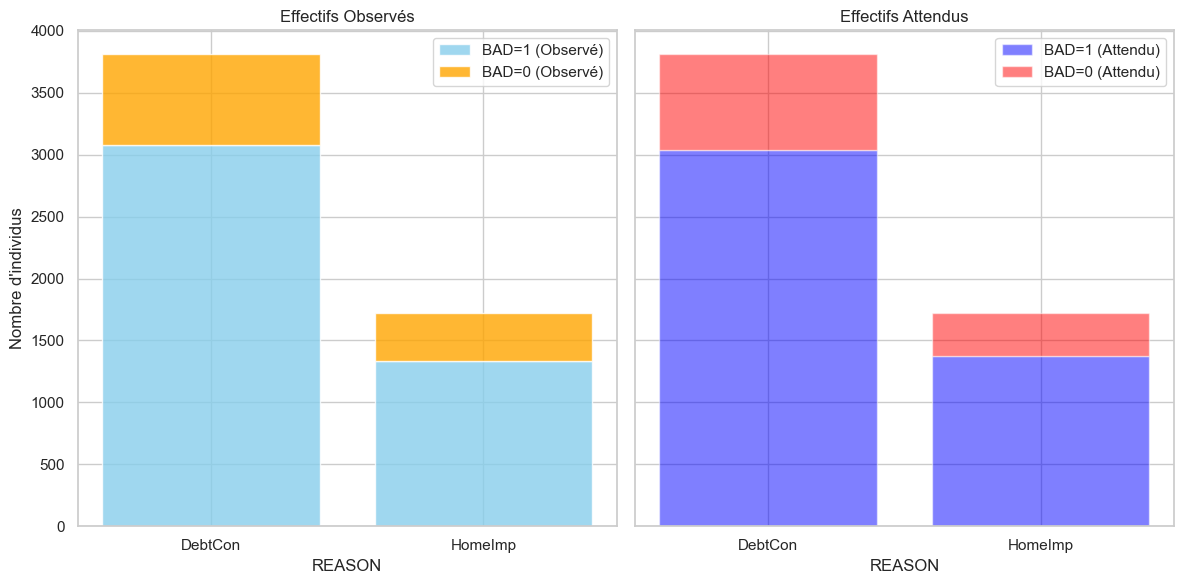
\includegraphics[width=\textwidth]{../images/plot_khi2_bad_vs_reason}
  \caption{Plot distribution des distributions observés vs attendues avec test du Khi 2, de BAD et REASON}
  \label{fig:plot_khi2_bad_vs_reason}
\end{figure}

On observe (Figure \ref{fig:plot_khi2_bad_vs_reason}) que l'effectif observé est presque égal à l'effectif attendu, et que la p-value est inférieure à 1\%. Par conséquent, on rejette $H_0$ au seuil de 1\%, ce qui indique une dépendance entre \texttt{BAD} et \texttt{REASON}.\\
C'est donc une bonne chose pour notre modèle que REASON puisse possiblement prédire BAD.

\subsubsection{Khi 2 entre {\color{teal} BAD} et {\color{teal} JOB}}

Après avoir effectué le test de Khi 2 entre {\color{teal} BAD} et {\color{teal} JOB}, nous obtenons les résultats suivants :\\

\begin{figure}[h!]
  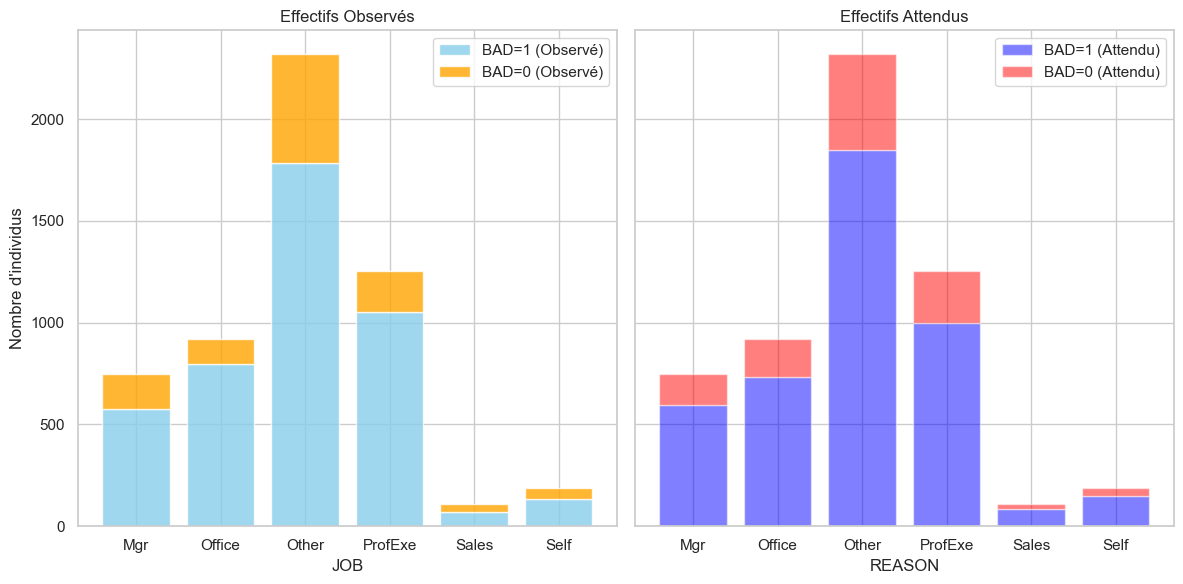
\includegraphics[width=\textwidth]{../images/plot_khi2_bad_vs_job}
  \caption{Plot distribution des distributions observés vs attendues avec test du Khi 2, de BAD et JOB}
  \label{fig:plot_khi2_bad_vs_job}
\end{figure}

\pagebreak

Les effectifs observés et attendus sont très proches (Figure \ref{fig:plot_khi2_bad_vs_job}), et la p-value calculée est inférieure à 1\%. Ainsi, nous rejetons $H_0$ au seuil de 1\%, ce qui met en évidence une relation de dépendance entre \texttt{BAD} et \texttt{JOB}.\\
Egalement, c'est donc une bonne chose pour notre modèle que JOB puisse possiblement prédire BAD.

\bigbreak

\textbf{Mais qu'en est-il de la relation entre REASON et JOB ?}\\

\begin{figure}[h!]
  \centering
  \begin{tabular}{|c|c|c|c|c|c|c|}
      \hline
      REASON/JOB & Other & Office & Sales & Mgr & ProfExe & Self \\
      \hline
      DebtCon & 513.82 & 634.35 & 1597.93 & 862.33 & 75.08 & 129.49 \\
      HomeImp & 232.18 & 286.65 & 722.07 & 389.67 & 33.92 & 58.51 \\
      \hline
  \end{tabular}
  \caption{Tableau des effectifs attendus entre \texttt{REASON} et les différentes catégories professionnelles.}
  \label{fig:table_khi2_reason_vs_job}
\end{figure}

\begin{figure}[h!]
  \centering
  \begin{tabular}{|c|c|c|c|c|c|c|}
      \hline
      REASON/JOB & Mgr & Office & Other & ProfExe & Sales & Self \\
      \hline
      DebtCon & 572 & 620 & 1604 & 847 & 97 & 73 \\
      HomeImp & 174 & 301 & 716 & 405 & 12 & 115 \\
      \hline
  \end{tabular}
  \caption{Tableau des effectifs observés entre \texttt{JOB} et les différentes catégories professionnelles.}
  \label{fig:table_khi2_reason_vs_job}
\end{figure}

\begin{figure}[h!]
  \centering
  \begin{tabular}{|l|c|}
      \hline
      \textbf{Statistique} & \textbf{Valeur} \\
      \hline
      Valeur p du test Khi² & $7.594 \times 10^{-25}$ \\
      Statistique Khi² & 122.91 \\
      Degrés de liberté & 5 \\
      Cramér's V & 0.1490023273179537 \\
      \hline
  \end{tabular}
  \caption{Résultats du test de Khi².}
  \label{fig:table_khi2_results_reason_vs_job}
\end{figure}

\pagebreak

Pour interpréter les valeurs du \textbf{V de Cramér} dans le tableau \ref{fig:table_khi2_results_reason_vs_job} :  
\begin{itemize}
    \item $0.0 - 0.1$ : Très faible association, les variables sont presque indépendantes.
    \item {\color{red} $0.1 - 0.3$ : Faible association.}
    \item $0.3 - 0.5$ : Moyenne association.
    \item $0.5 - 0.7$ : Forte association.
    \item $0.7 - 1.0$ : Très forte association.
\end{itemize}

\bigbreak

Finalement, avec le test de Khi², nous avons constaté que les deux variables explicatives catégorielles \texttt{REASON} et \texttt{JOB} sont dépendantes 
puisqu'on a un p-value nettement inférieur à 1\%.\\
De plus, lorsqu'on vérifie la force de l'association entre ces deux variables avec le V de Cramér, nous obtenons une valeur de $0.14$, ce qui correspond à une association faible.

Compte tenu de la force du rejet de $H_0$ dans le test de significativité d'indépendance entre \texttt{BAD} $\leftarrow$ \texttt{JOB} et \texttt{BAD} $\leftarrow$ \texttt{REASON}, \texttt{JOB} a été rejetée avec beaucoup plus de confiance que la variable \texttt{REASON}. Nous pouvons donc supprimer la variable \texttt{REASON}, car elle pourrait avoir un lien de prédiction avec \texttt{BAD} moins important que \texttt{JOB}.

\pagebreak

\section{Modélisation}

Après tout le processus de sélection des variables explicatives (\textit{feature selection}), nous obtenons le modèle suivant :  
\[
\texttt{BAD} \leftarrow \texttt{LOAN}, \texttt{MORTDUE}, \texttt{JOB}, \texttt{YOJ}, \texttt{DEROG}, \texttt{DELINQ}, \texttt{CLAGE}, \texttt{NINQ}
\]

Nous pouvons donc passer au test de plusieurs modèles de classification avec les meilleurs paramètres.  
Pour cela, nous utiliserons les métriques que nous avons choisies afin d'évaluer ces différents modèles.


\subsection{Métriques de performances}

Il existe plusieurs façons d’évaluer la performance d’un modèle de classification. Parmi les métriques courantes figurent la précision (\textit{accuracy}), la précision au sens strict, le rappel (\textit{recall}), le F1-score et l’AUC ROC. Chaque métrique met en évidence un aspect spécifique des performances, qu’il s’agisse de l’exactitude globale ou de l’équilibre entre les faux positifs et les faux négatifs. Le choix des métriques pertinentes dépend des exigences spécifiques du problème.
\bigbreak
Dans ce projet, nous avons décidé de privilégier le \textit{recall} comme métrique principale et l’AUC ROC comme métrique secondaire.
\bigbreak
Dans le contexte des approbations de prêts, le \textit{recall} est particulièrement important car il mesure la proportion de mauvais payeurs (\texttt{BAD} = 1) identifiés correctement par le modèle. Mal classer ces individus comme peu risqués (faux négatifs) représente un risque financier majeur pour les prêteurs. Ce risque dépasse le coût des faux positifs (classer par erreur un bon payeur comme mauvais), car les pertes potentielles dues aux défauts de paiement sont généralement bien supérieures aux bénéfices perdus en refusant un demandeur solvable.

\bigbreak
\textbf{Définition et calcul du rappel}
\smallbreak
Le \textit{recall}, ou sensibilité, mesure la capacité à identifier tous les mauvais payeurs (\texttt{BAD} = 1). Il est calculé ainsi :
\[Recall = \frac{True Positive}{True Positive + False Negative}\]
Un \textit{recall} élevé garantit que la majorité des emprunteurs à risque sont identifiés, minimisant ainsi les pertes financières.

\pagebreak
\subsection{Dataset}

Tous les modèles ont été développés et évalués sur deux jeux de données principaux: les données brutes et les données transformées.

\subsubsection{Les données brutes (Raw Data)}
Ce jeu de données représente les données d'origine, où toutes les variables initiales sont conservées. Les valeurs manquantes (\texttt{NaN}) ont été simplement supprimées sans aucune autre manipulation. Cela permet de servir de référence pour comparer les performances des modèles sur un jeu de données minimalement prétraité. Ce choix garantit une base pour évaluer l'impact des transformations ultérieures.

\subsubsection{Les données transformées (Processed Data)}
Ce jeu de données inclut l'ensemble des transformations et améliorations apportées lors de l'étape de prétraitement.

\subsection{Balancement des classes}

Un déséquilibre notable existe entre les classes dans la variable cible \texttt{BAD} (19,9\% de défauts contre 80,1\% de non-défauts). Ce déséquilibre peut biaiser les modèles en favorisant la classe majoritaire (\texttt{BAD} = 0). Pour y remédier :

\begin{itemize}
  \item \textbf{SMOTE} (Synthetic Minority Oversampling Technique) a été appliqué à certains modèles pour augmenter artificiellement le nombre d'observations dans la classe minoritaire (\texttt{BAD} = 1).
  \item \textbf{Rééquilibrage des poids des classes} (\texttt{class\_weight}) a également été utilisé dans des modèles tels que la régression logistique et la forêt aléatoire, permettant de pénaliser davantage les erreurs sur la classe minoritaire.
\end{itemize}

\subsection{Baseline Modeling (Benchmark) : KNN et Naive Bayes}

Pour établir une base de référence, deux modèles simples ont été utilisés : K-Nearest Neighbors (KNN) et Naive Bayes. Ces modèles ont été appliqués aux deux jeux de données (bruts et transformés) pour évaluer leurs performances initiales. Voici les résultats obtenus (Table \ref{table:benchmark_model}) :

\begin{table}[h!]
  \centering
  \begin{tabular}{|l|c|c|}
    \hline
    \textbf{Modèle} & \textbf{AUC} & \textbf{Rappel} \\
    \hline
    KNN Transformé & 0.629 & 0.181 \\
    \hline
    KNN Raw & 0.625 & 0.097 \\
    \hline
    Naive Bayes Transformé & 0.738 & 0.177 \\
    \hline
    Naive Bayes Raw & 0.804 & 0.226 \\
    \hline
  \end{tabular}
  \caption{Résultats des modèles de base : KNN et Naive Bayes}
  \label{table:benchmark_model}
\end{table}

\subsubsection{Résultats des modèles}

\begin{itemize}
  \item{ \textbf{KNN} \newline
    Ce modèle, bien qu'assez intuitif, présente des performances relativement faibles en termes de rappel, surtout avec les données brutes. Cela peut s'expliquer par une sensibilité accrue aux dimensions et à la répartition des données. Le rappel plus élevé sur les données transformées indique que les étapes de prétraitement, telles que l'imputation et la sélection des caractéristiques, améliorent la capacité du modèle à identifier la classe minoritaire.
    }
  \item{ \textbf{Naive Bayes} \newline
    Ce modèle montre des performances meilleures que KNN, notamment en termes d'AUC, avec une nette amélioration sur les données brutes. Cela reflète la capacité de Naive Bayes à bien gérer les données brutes, probablement grâce à l'hypothèse d'indépendance conditionnelle qui réduit l'impact des relations entre les variables.
  }
\end{itemize}

\chapter{Classifications, résultats et conclusion}

\section{Approche Générale de la Modélisation}

Pour standardiser et simplifier le processus de modélisation, nous avons développé une fonction polyvalente, \texttt{train\_test\_with\_cv}. Cette fonction automatise l'optimisation des hyperparamètres, l'évaluation des modèles et l'ajustement des seuils, garantissant ainsi une cohérence dans l'ensemble des modèles tout en offrant une flexibilité pour les ajustements spécifiques. Voici un aperçu de ses principales composantes et de son implémentation :

\begin{itemize}
  \item La fonction utilise \texttt{GridSearchCV} pour l'optimisation des hyperparamètres, en testant les combinaisons spécifiées dans la grille (\texttt{param\_grid}) à l'aide de la validation croisée (\texttt{cv}).
  \item Elle refait automatiquement l'apprentissage du meilleur modèle sur les données d'entraînement après avoir identifié les paramètres optimaux.
  \item Une fois le modèle ajusté, elle évalue les performances sur les ensembles d'entraînement et de test, en calculant des métriques telles que l'AUC, l'exactitude pondérée et le rappel, offrant ainsi une compréhension complète des performances du modèle.
  \item Si un modèle prend en charge \texttt{predict\_proba} ou \texttt{decision\_function}, ces sorties sont utilisées pour calculer les métriques et ajuster les seuils de manière précise.
  \item Une fonctionnalité clé réside dans la gestion des seuils personnalisés, particulièrement utile pour les jeux de données déséquilibrés.
  \item La fonction accepte un paramètre \texttt{threshold} pour ajuster la frontière de décision pour la classification. Les métriques telles que le rappel, la précision et le score F1 sont recalculées en fonction des prédictions ajustées.
  \item La fonction visualise également les performances via des courbes ROC, illustrant la sensibilité et la spécificité, et génère des matrices de confusion pour évaluer l'impact des seuils personnalisés sur les décisions de classification.
\end{itemize}

\section{Algorithmes de Modélisation}

Nous avons utilisé une gamme d'algorithmes avancés pour garantir des prédictions robustes et gérer efficacement le déséquilibre inhérent des classes dans le jeu de données. Voici une description détaillée des principaux algorithmes utilisés, leur fonctionnement et leur pertinence dans notre contexte.

\subsection{Random Forest}

La \textit{Forêt Aléatoire} est un algorithme d'apprentissage ensembliste qui construit plusieurs arbres de décision pendant l'entraînement et agrège leurs prédictions (par vote majoritaire pour les tâches de classification). Chaque arbre est entraîné sur un sous-ensemble aléatoire des données et des caractéristiques, ce qui réduit le surapprentissage et améliore la généralisation.

Cet algorithme est particulièrement adapté à notre projet car il est robuste face au surapprentissage, ce qui le rend efficace même pour les jeux de données contenant du bruit ou des structures complexes. De plus, il peut gérer les valeurs manquantes sans nécessiter de prétraitement intensif, un atout pour notre jeu de données brut. Enfin, sa capacité à capturer les relations non linéaires en fait un choix puissant pour améliorer la précision prédictive.

\subsubsection{Résultats et Analyse}

Avec les données transformées, la \textit{Forêt Aléatoire} a démontré une augmentation notable du rappel sur l'ensemble de test, atteignant 82,7\% avec un seuil ajusté (0.4). Cet ajustement de seuil a permis de prioriser la détection des individus à risque (classe positive) tout en maintenant une bonne performance globale mesurée par l'AUC ROC.

La matrice de confusion des données transformées montre que, bien que le modèle ait correctement identifié de nombreux cas positifs, une proportion non négligeable de faux positifs (213) persiste. Ce comportement est justifiable dans des scénarios où le rappel est prioritaire.
\bigbreak
Pour les données brutes, le modèle a surpassé les résultats obtenus avec les données transformées en termes de rappel. Cela met en évidence la capacité des Forêts Aléatoires à exploiter efficacement des données non traitées, en tirant parti des relations naturelles dans le jeu de données brut. Cependant, la matrice de confusion révèle que la détection des cas positifs s'est légèrement améliorée, avec une réduction significative des faux négatifs par rapport aux données transformées.

Dans les deux cas, les performances élevées en termes de rappel et d'AUC ROC confirment que la \textit{Forêt Aléatoire} est bien adaptée à ce projet.

\subsection{Régression Logistique}

La \textit{Régression Logistique} a été choisie pour sa simplicité, son efficacité en classification binaire et sa capacité à fournir une interprétation claire des relations entre les caractéristiques et la classe cible. Elle est particulièrement adaptée aux jeux de données avec un déséquilibre des classes grâce à la possibilité d'intégrer des pondérations.

Ce modèle a été utilisé à la fois sur les données transformées et brutes. Contrairement aux modèles comme la \textit{Forêt Aléatoire}, la Régression Logistique n’est pas directement adaptée à l’utilisation de seuils personnalisés. Ce modèle effectue des prédictions basées sur une probabilité linéaire, où le seuil par défaut de 0.5 est utilisé. Ainsi, l'ajustement des seuils n'était pas pertinent dans ce cas.
\bigbreak
Le modèle a présenté une AUC test de 0.736 et un rappel de 0.642 sur les données transformées. Sur les données brutes, le modèle a légèrement surpassé ces résultats avec un rappel de 0.710. Bien qu'il ne s'agisse pas des meilleures performances globales, la \textit{Régression Logistique} a montré un excellent équilibre en étant le modèle le moins sujet au surapprentissage. Les matrices de confusion révèlent que les données brutes ont permis une meilleure détection des cas positifs tout en maintenant un équilibre satisfaisant entre faux positifs et vrais positifs.

\subsection{Support Vector Machines}

Les \textit{Support Vector Machines} (SVM) classent les données en identifiant l’hyperplan qui maximise la marge entre les classes. Les relations non linéaires sont gérées via des fonctions noyau, telles que le noyau radial (RBF). Cet algorithme est idéal pour les jeux de données à caractéristiques de haute dimension. Sa flexibilité dans le choix du noyau lui permet de s’adapter à divers motifs présents dans les données, offrant ainsi une capacité de classification robuste et précise.

Contrairement à d'autres modèles, nous n'avons pas appliqué de seuils personnalisés avec les SVM. Cela s'explique par la façon dont les SVM produisent des scores de décision plutôt que des probabilités directement. Ces scores ne peuvent pas être interprétés comme des probabilités standard, ce qui rend difficile l'application d'un seuil comparable à celui utilisé dans les autres modèles.

\subsubsection{Performances sur les Données Transformées et Brutes}

Sur les données transformées, le modèle a obtenu une AUC de 0.869 et un rappel de 0.704 sur le test. Les données brutes, cependant, ont montré une amélioration de l'AUC test, atteignant 0.900. Toutefois, le rappel sur ces données était légèrement inférieur, à 0.677. Les résultats indiquent que le modèle a légèrement mieux capturé les motifs présents dans les données transformées pour détecter les cas positifs, tandis que les données brutes ont permis une meilleure séparation globale des classes.

\subsection{Gradient Boosting}

Le \textit{Gradient Boosting} construit des arbres de décision séquentiels, chacun corrigeant les erreurs de son prédécesseur. L’algorithme optimise une fonction de perte, telle que la log-perte, en affinant les prédictions de manière itérative.

Il capture efficacement les motifs complexes et les interactions dans les données, ce qui est essentiel pour notre projet. La flexibilité dans l’ajustement des hyperparamètres, tels que le taux d’apprentissage et la profondeur des arbres, permet un contrôle précis de la complexité du modèle. Comme cet algorithme ne gère pas nativement le déséquilibre des classes, nous avons intégré SMOTE (Synthetic Minority Oversampling Technique) dans le pipeline.

\subsubsection{Analyse des Résultats}

Sur les données transformées, le \textit{Gradient Boosting} a montré une AUC de 0.895 et un rappel de 0.478, indiquant une tendance conservatrice qui favorise les prédictions négatives, comme le reflète la matrice de confusion. Sur les données brutes, le modèle a présenté une AUC légèrement meilleure, mais un rappel plus faible de 0.387, confirmant un surapprentissage (\textit{overfitting}) et une mauvaise généralisation sur des données non vues. Avec l’intégration de SMOTE, le rappel a été significativement amélioré à 0.673, mais au prix d'une baisse de l’AUC. Cette approche a permis un équilibre dans la détection des cas positifs, bien qu’elle ait introduit davantage de faux positifs.

\section{Tableau des résultats}

\begin{table}[h!]
  \centering
  \begin{tabular}{|l|l|c|c|c|}
  \hline
  \textbf{Modèle} & \textbf{Type de données} & \textbf{Recall} & \textbf{AUC (test)} & \textbf{Threshold} \\
  \hline
  Random Forest & Processed & 0.827 & 0.891 & 0.4 \\
  Random Forest & Raw & 0.839 & 0.904 & 0.45 \\
  Logistic Regression & Processed & 0.642 & 0.736 & 0.5 \\
  Logistic Regression & Raw & 0.710 & 0.778 & 0.5 \\
  SVM & Processed & 0.704 & 0.869 & 0.5 \\
  SVM & Raw & 0.677 & 0.900 & 0.5 \\
  Gradient Boosting & Processed & 0.478 & 0.895 & 0.5 \\
  Gradient Boosting & Raw & 0.387 & 0.928 & 0.5 \\
  Smote & Processed & 0.673 & 0.732 & 0.5 \\
  \hline
  \end{tabular}
  \caption{Résultats des modèles}
  \label{tab:results_models}
\end{table}

Parmi les différents modèles testés, en regardant le tableau récapitulatif des résultats des modèles (Table \ref{tab:results_models}), \textbf{Random Forest} avec les données brutes (\textit{raw}) a fourni les meilleurs résultats en termes de \textbf{Recall} (0.839) et d'\textbf{AUC} (Test) (0.904), tout en maintenant un seuil de 0.45. Ces performances indiquent que ce modèle est particulièrement efficace pour détecter les cas positifs tout en offrant une bonne discrimination entre les classes. 

Le \textbf{Random Forest} est souvent performant dans ce type de scénario grâce à :
\begin{itemize}
    \item sa capacité à gérer la complexité des données,
    \item sa réduction du surapprentissage grâce à l’agrégation de nombreux arbres,
    \item sa robustesse face aux données brutes (\textit{raw data}).
\end{itemize}

\bigbreak

En revanche, bien que d'autres modèles, comme le \textbf{Gradient Boosting}, aient montré un AUC légèrement supérieur avec les données brutes (0.928), leur \textbf{Recall} plus faible (0.387) les rend moins adaptés lorsque la détection des cas positifs est critique, comme c'est souvent le cas dans les systèmes de classification où les faux négatifs doivent être minimisés. 

Ainsi, le \textbf{Random Forest} avec les données brutes se démarque comme le modèle offrant le meilleur compromis entre sensibilité et précision globale.

\pagebreak

\section*{Conclusion}

Le projet a permis de mettre en pratique des concepts clés en analyse de données et en modélisation prédictive pour résoudre un problème réel lié au scoring de risque de crédit. À travers l'utilisation des données HMEQ, nous avons exploré diverses étapes cruciales, allant de l'analyse exploratoire des données, au traitement des valeurs manquantes et des outliers, jusqu’à la construction et l’évaluation de plusieurs modèles de machine learning.

Parmi les modèles testés, \textbf{la forêt aléatoire} s'est révélée être le plus performant, avec une capacité remarquable à détecter les cas de défaut tout en maintenant une bonne capacité discriminative globale. Les techniques de rééquilibrage des classes, telles que \textbf{SMOTE}, ainsi que les ajustements des seuils de décision, ont joué un rôle crucial pour gérer l’aspect déséquilibré de la variable cible. Ces approches ont permis d'optimiser la sensibilité des modèles, un objectif essentiel dans le contexte de la gestion des risques financiers.

\bigbreak

Le projet met également en lumière l'importance du choix des métriques d’évaluation adaptées au problème traité. En privilégiant le \textbf{rappel} comme indicateur principal, nous avons pu prioriser la minimisation des faux négatifs, réduisant ainsi le risque pour les institutions prêteuses.

Enfin, ce projet nous a offert une opportunité précieuse d’appliquer nos connaissances théoriques à une problématique concrète, renforçant ainsi notre compréhension des enjeux liés au scoring dans le secteur bancaire et financier. Nous en ressortons non seulement enrichis sur le plan technique, mais aussi sensibilisés aux responsabilités éthiques et stratégiques associées à l’analyse prédictive.



\pagebreak
\appendix
\section{Annexe : Distribution des variables numériques}

\begin{figure}[h!]
  \centering
  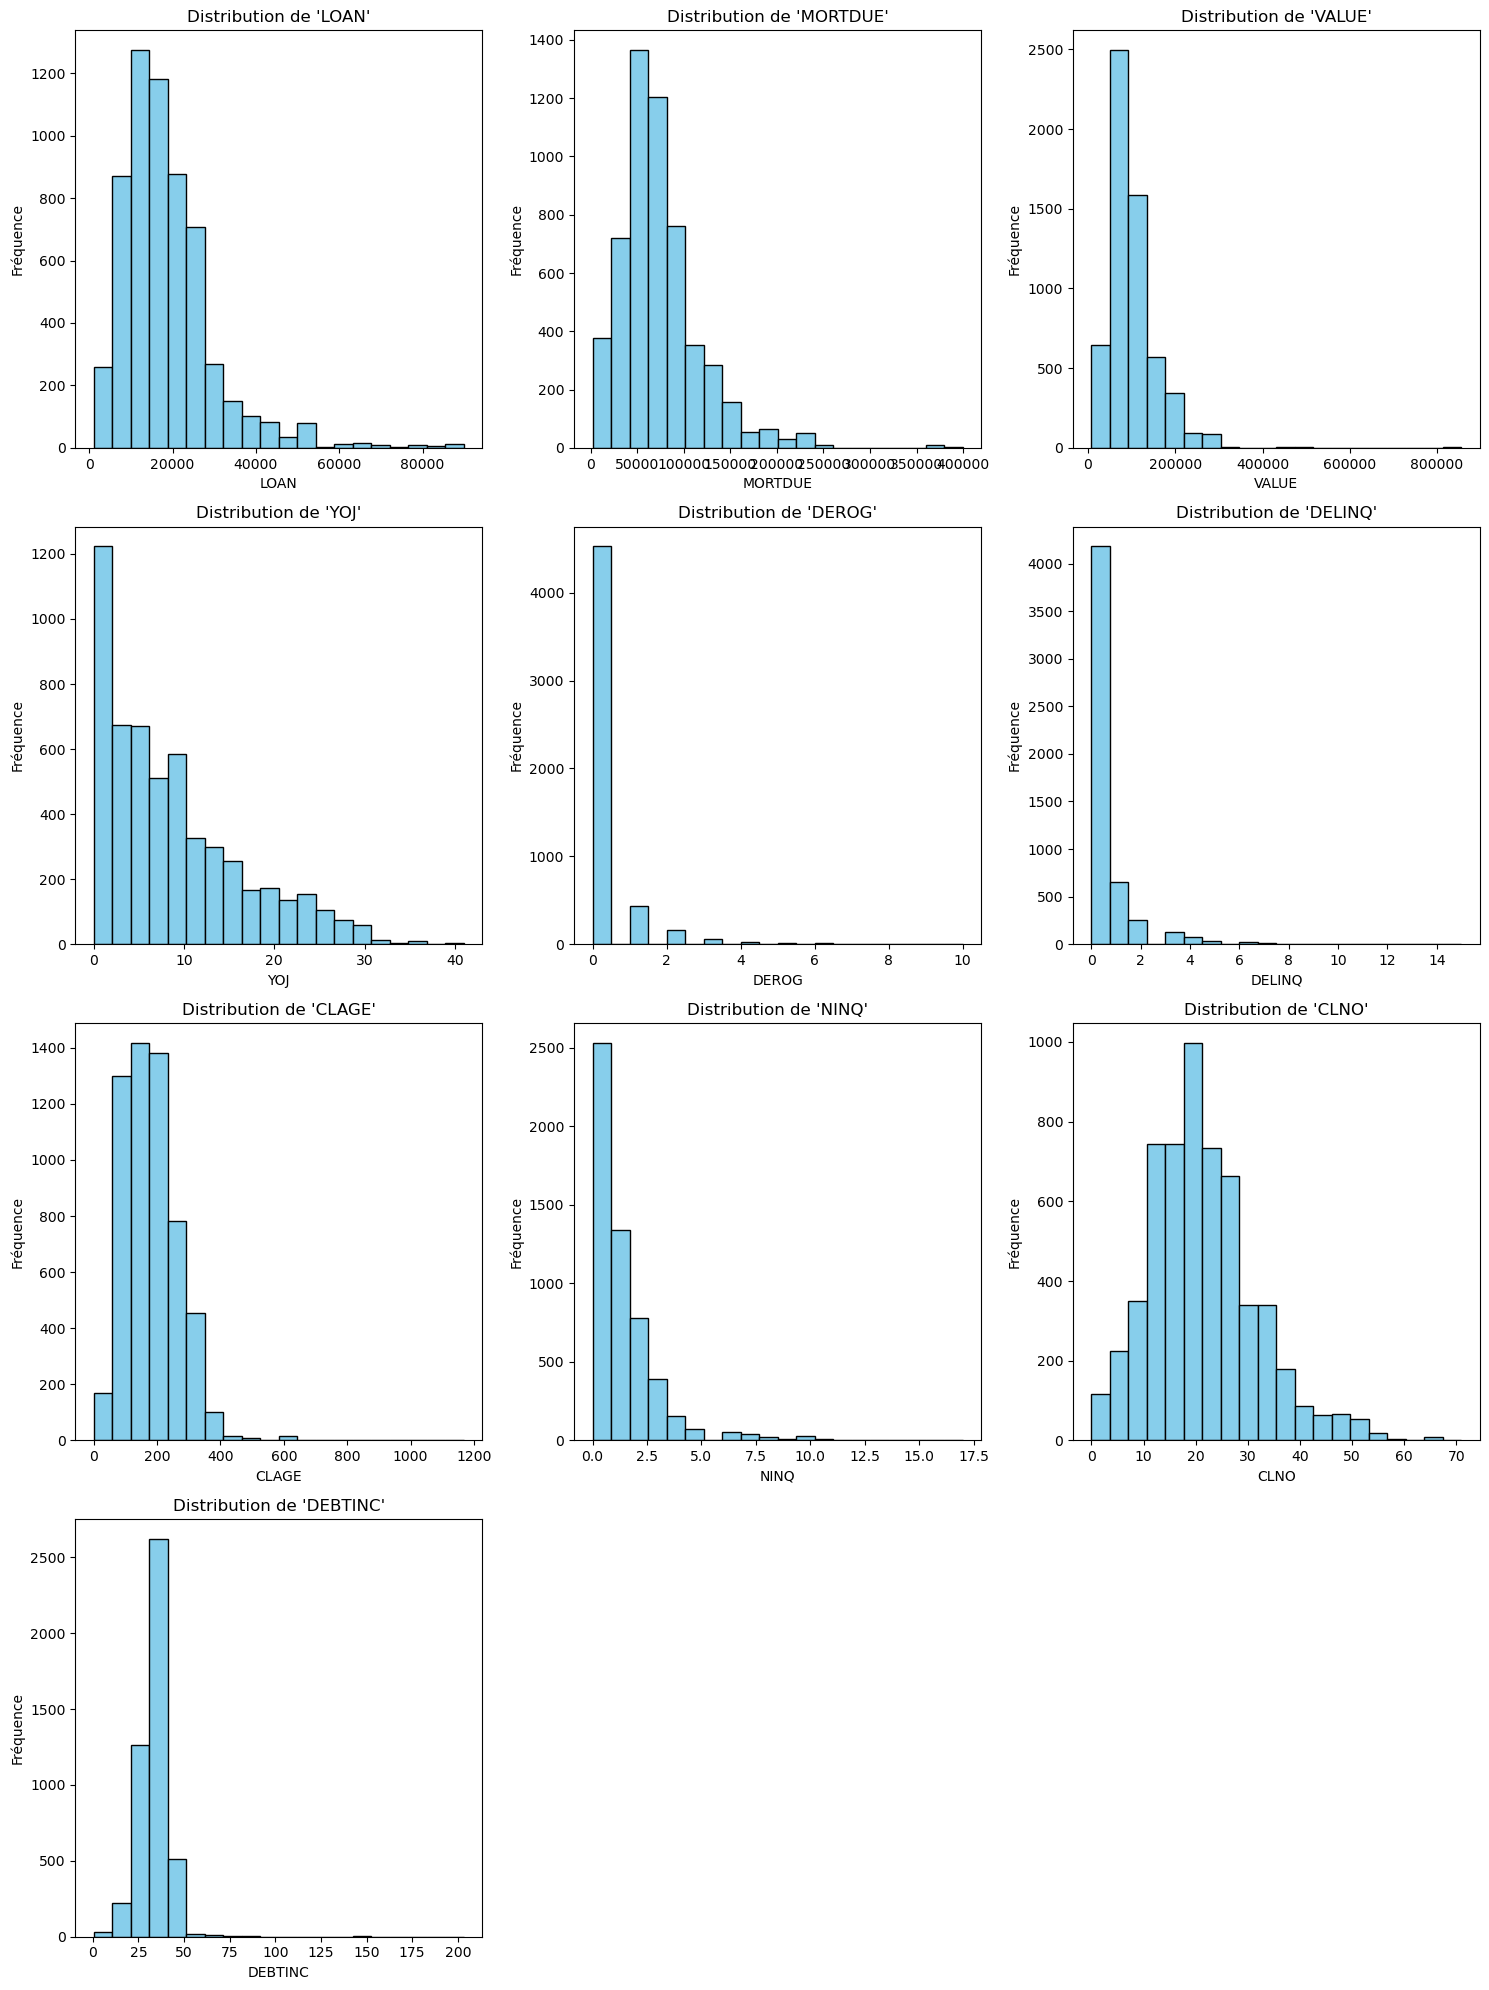
\includegraphics[width=\textwidth]{../images/plot_dist_num_data}
  \label{fig:plot_dist_num_data}
\end{figure}

\section{Annexe : Barplot de JOB par rapport à BAD}
\begin{figure}[h!]
  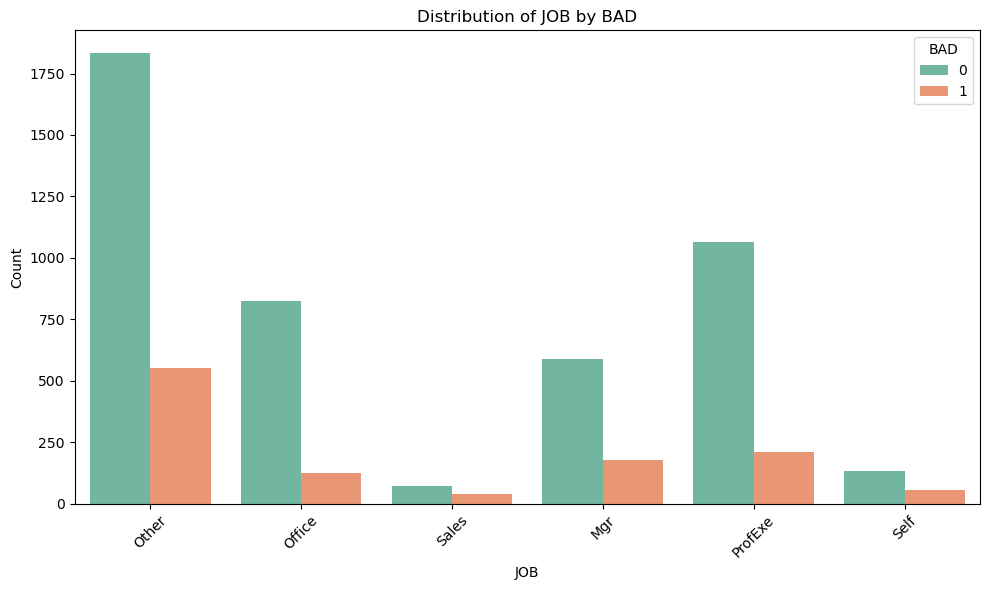
\includegraphics[width=\textwidth]{../images/barplot_job_by_bad}
  \label{fig:barplot_job_by_bad}
\end{figure}

\section{Annexe : Barplot de REASON par rapport à BAD}
\begin{figure}[h!]
  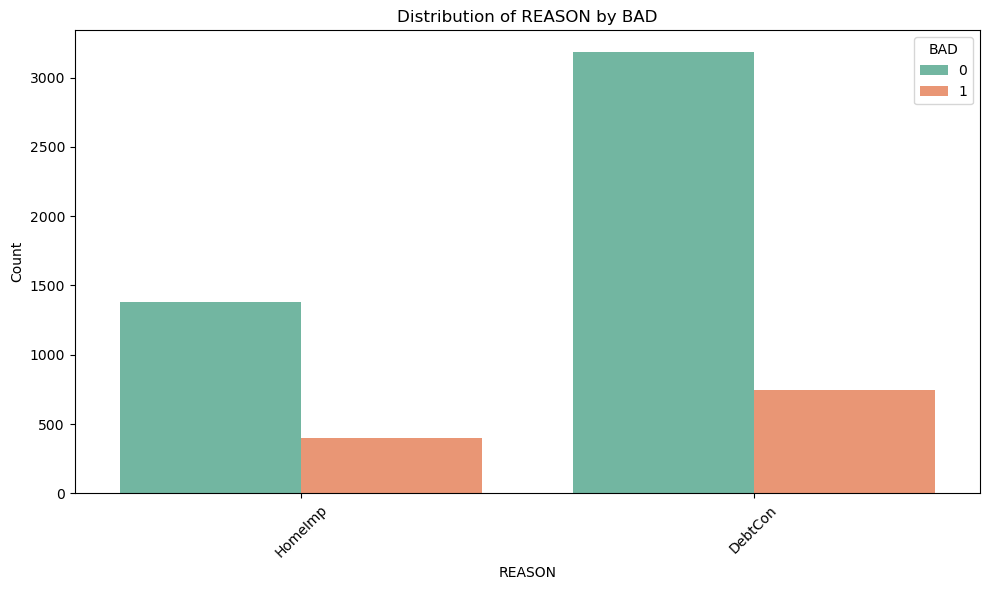
\includegraphics[width=\textwidth]{../images/barplot_reason_by_bad}
  \label{fig:barplot_reason_by_bad}
\end{figure}

\section{Annexe : Boxplot des variables numériques par rapport à BAD}

\begin{figure}[h!]
  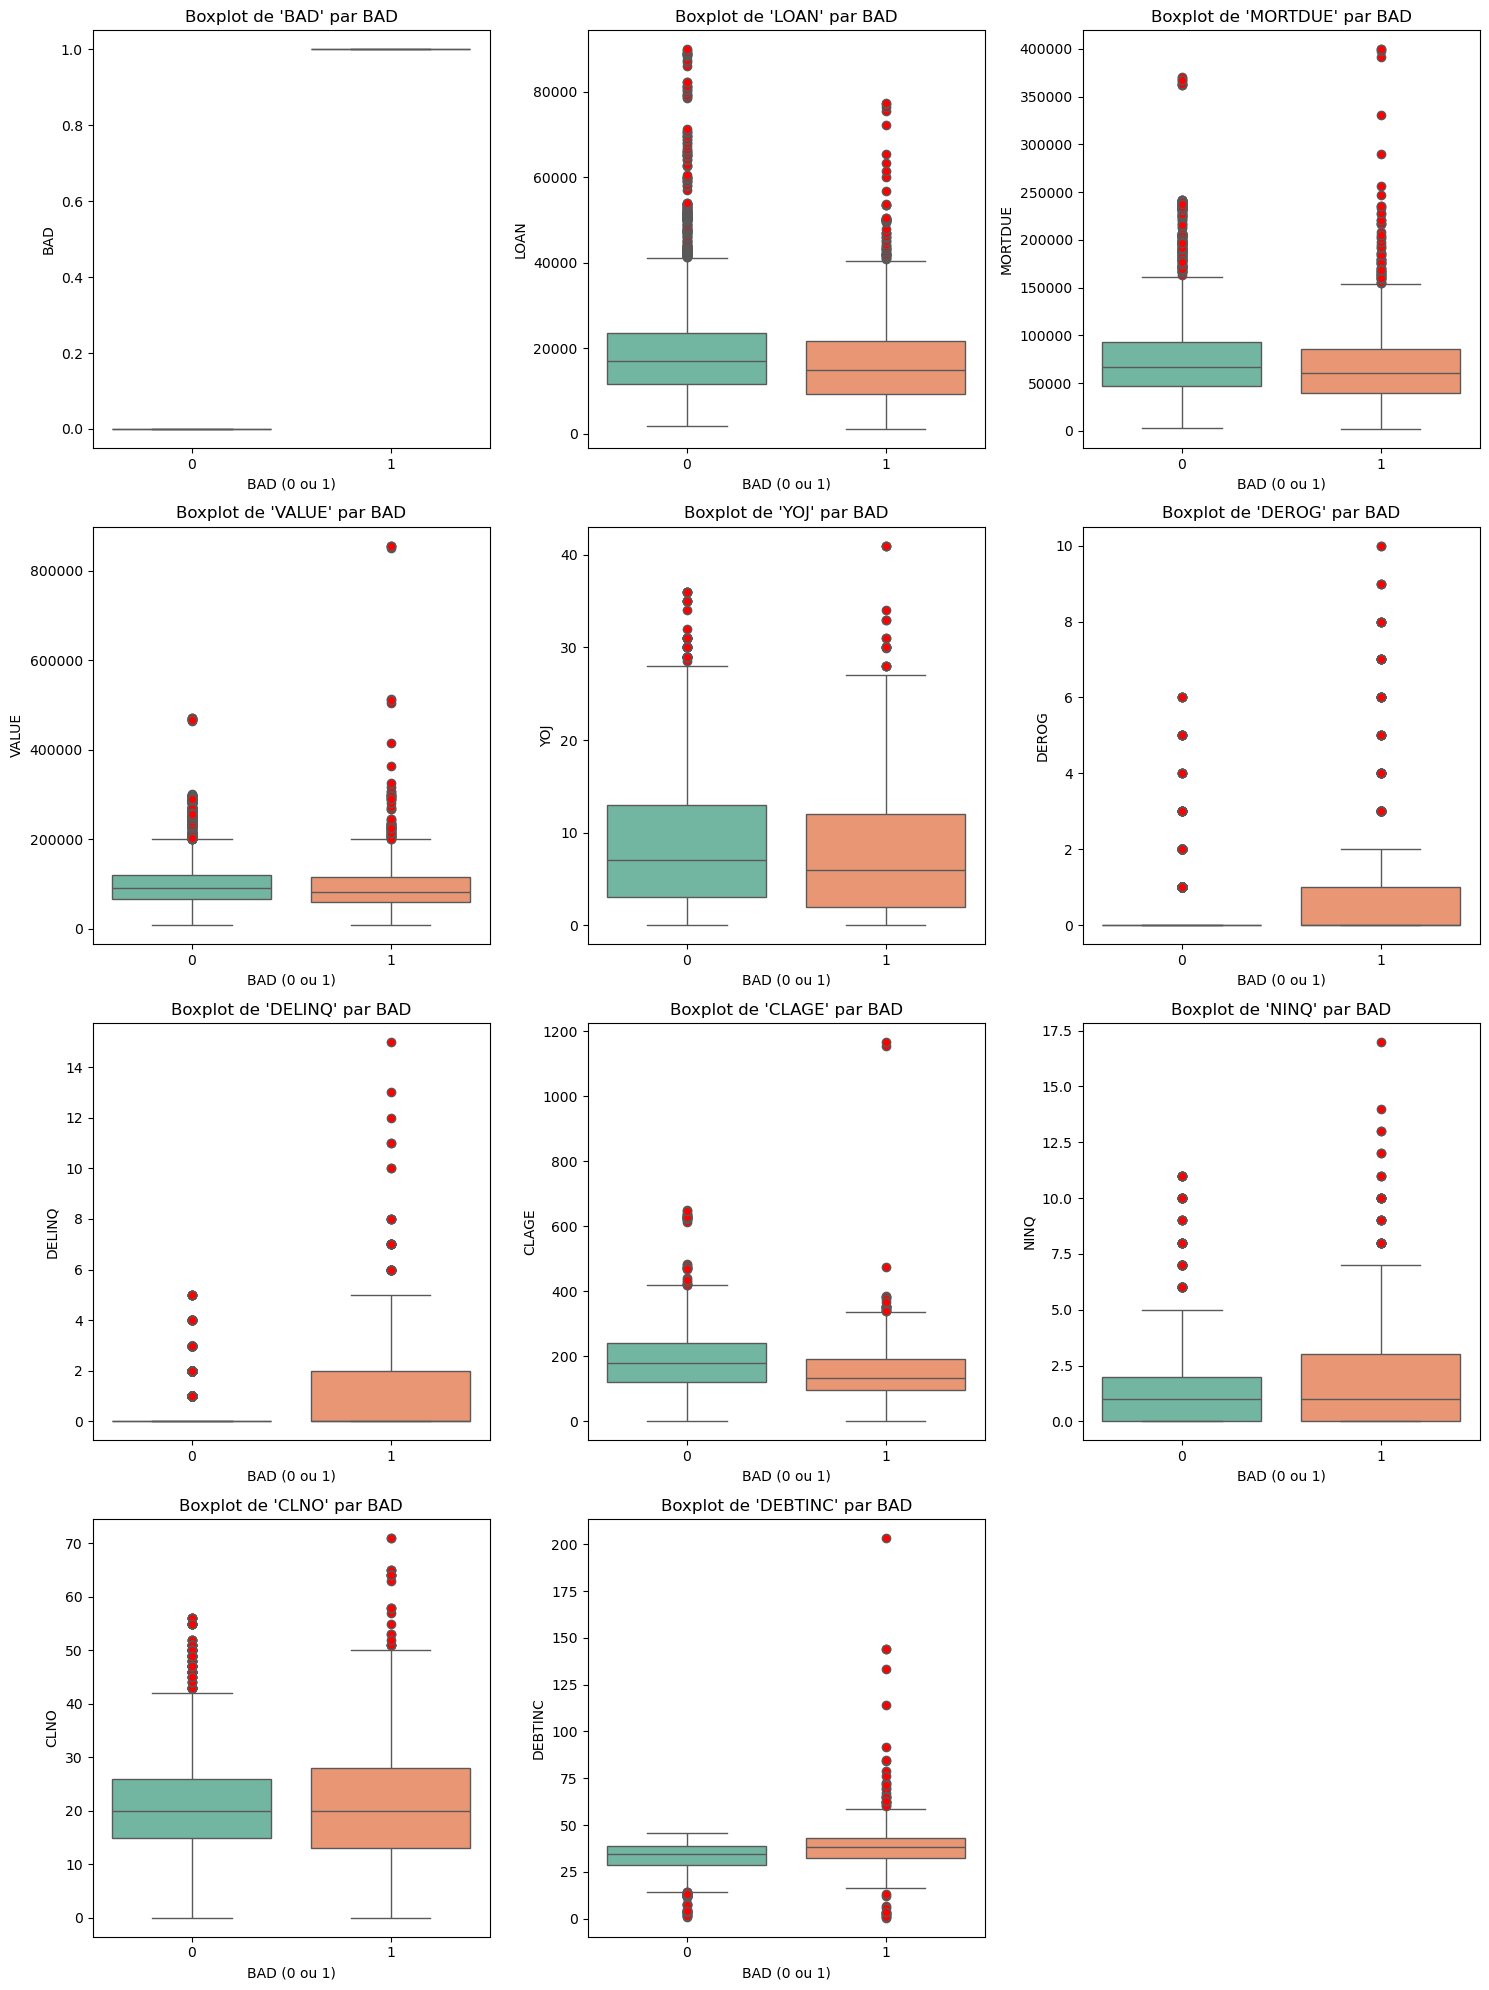
\includegraphics[width=\textwidth]{../images/boxplot_var_num}
  \label{fig:boxplot_var_num}
\end{figure}


\end{document}
